% -*- mode: LaTeX; TeX-PDF-mode: t; -*- 
% LaTeX path to the root directory of the current project
% from the directory in which this file resides
% and path to econtexPaths which defines the rest of the paths like \FigDir
\providecommand{\econtexRoot}{}\renewcommand{\econtexRoot}{.}
\providecommand{\econtexPaths}{}\renewcommand{\econtexPaths}{econtexPaths}
% -*- mode: LaTeX; TeX-PDF-mode: t; -*- 
% The \commands below are required to allow sharing of the same base code via Github between TeXLive on a local machine and Overleaf (which is a proxy for "a standard distribution of LaTeX").  This is an ugly solution to the requirement that custom LaTeX packages be accessible, and that Overleaf prohibits symbolic links
\providecommand{\packages}{\econtexRoot/Resources/texmf-local/tex/latex}
\providecommand{\econtex}{\packages/econtex}
\providecommand{\econark}{\econtexRoot/Resources/texmf-local/tex/latex/econark}
\providecommand{\econtexSetup}{\econtexRoot/Resources/texmf-local/tex/latex/econtexSetup}
\providecommand{\econarkSetup}{\econtexRoot/Resources/texmf-local/tex/latex/econarkSetup}
\providecommand{\econtexShortcuts}{\econtexRoot/Resources/texmf-local/tex/latex/econtexShortcuts}
\providecommand{\econtexBibMake}{\econtexRoot/Resources/texmf-local/tex/latex/econtexBibMake}
\providecommand{\econtexBibStyle}{\econtexRoot/Resources/texmf-local/bibtex/bst/econtex}
\providecommand{\econtexBib}{economics}
\providecommand{\notes}{\econtexRoot/Resources/texmf-local/tex/latex/handout}
\providecommand{\handoutSetup}{\econtexRoot/Resources/texmf-local/tex/latex/handoutSetup}
\providecommand{\handoutShortcuts}{\econtexRoot/Resources/texmf-local/tex/latex/handoutShortcuts}
\providecommand{\handoutBibMake}{\econtexRoot/Resources/texmf-local/tex/latex/handoutBibMake}
\providecommand{\handoutBibStyle}{\econtexRoot/Resources/texmf-local/bibtex/bst/handout}

\providecommand{\FigDir}{\econtexRoot/Figures}
\providecommand{\CodeDir}{\econtexRoot/Code}
\providecommand{\DataDir}{\econtexRoot/Data}
\providecommand{\SlideDir}{\econtexRoot/Slides}
\providecommand{\TableDir}{\econtexRoot/Tables}
\providecommand{\ApndxDir}{\econtexRoot/Appendices}

\providecommand{\ResourcesDir}{\econtexRoot/Resources}
\providecommand{\rootFromOut}{..} % APFach back to root directory from output-directory
\providecommand{\LaTeXGenerated}{\econtexRoot/LaTeX} % Put generated files in subdirectory
\providecommand{\econtexPaths}{\econtexRoot/Resources/econtexPaths}
\providecommand{\LaTeXInputs}{\econtexRoot/Resources/LaTeXInputs}
\providecommand{\LtxDir}{LaTeX/}
\providecommand{\EqDir}{\econtexRoot/Equations} % Put generated files in subdirectory

\providecommand{\titlepagecustom}{\LaTeXInputs/titlepagecustom}


\documentclass[pdflatex,aspectratio=169]{beamer}
\usepackage{HAFiscal-Slides.pdf}
\usepackage{multirow}

%[notes,10pt,dvipsnames,aspectratio=169]

\newbool{buffstk}\global\boolfalse{buffstk}%\booltrue{buffstk}%\boolfalse{buffstk}
\newbool{bristol}\global\boolfalse{bristol}%\booltrue{bristol}%\boolfalse{bristol}
\newbool{bundesb}\global\boolfalse{bundesb}%\booltrue{bundesb}%\boolfalse{bundesb}
\newbool{omg}\global\booltrue{omg}%\boolfalse{omg}
\usepackage{\econark,\econtexShortcuts}

% _____________ Opening slide _______________________

\ifbool{buffstk}{% For bufferstock paper
  \title[Buffer Stock Theory]{Theoretical Foundations of Buffer Stock Saving}
  \author[Carroll]{Chris Carroll}
  \institute[JHU]{Johns Hopkins University}
  \date[\today]{September 12, 2019  \\ \medskip \medskip \medskip \href{https://econ-ark.org/}{\small Powered By} \\ 
\includegraphics[width=0.5in]{econ-ark-logo-small.png}}
}{}


\title[Stimulus]{Welfare and Spending Effects of Consumption Stimulus Policies}
\author{
  Christopher D. Carroll
  \and
  Edmund Crawley
  \and \\
  Ivan Frankovic
  \and
  H{\aa}kon Tretvoll
}

\ifbool{bristol}{% set date for bristol presentation
  \date[\today]{September 12, 2019  \\ \medskip \medskip \medskip \href{https://econ-ark.org/}{\small Powered By} \\ 
\includegraphics[width=0.5in]{econ-ark-logo-small.png}}
}{}

\ifbool{bundesb}{% set date for bundesbank
  \date[\today]{September 12, 2019  \\ \medskip \medskip \medskip \href{https://econ-ark.org/}{\small Powered By} \\ 
\includegraphics[width=0.5in]{econ-ark-logo-small.png}}
}{}

\ifbool{omg}{% set date for Oslo Macro Group
	%\institute{Oslo Macro Group}
	\date[\today]{Oslo Macro Group, February 14, 2023  \\ \medskip \medskip \medskip 
	\href{https://econ-ark.org/}{\small Powered By} \\ 
\includegraphics[width=0.5in]{econ-ark-logo-small.png}}
}{}


\newcommand{\RNum}[1]{\uppercase\expandafter{\romannumeral #1\relax}}
\newcommand{\ra}{\ensuremath{\Rightarrow}}
\newcommand{\myred}[1]{\textcolor{red}{#1}}
\newcommand{\myblue}[1]{\textcolor{blue}{#1}}

\AtBeginSection[]{
	\begin{frame}
	\vfill
	\centering
	\begin{beamercolorbox}[sep=8pt,center,shadow=true,rounded=true]{title}
		\usebeamerfont{title}\insertsectionhead\par%
	\end{beamercolorbox}
	\vfill
\end{frame}
}

\usepackage[font=small,skip=0pt]{caption}
\usepackage{booktabs}

\begin{document}\bibliographystyle{econark}

\begin{frame}[plain]
  \titlepage

\footnotesize{Viewpoints and conclusions stated in this paper are the responsibility of the authors alone and do not necessarily reflect the viewpoints of The Federal Reserve Board or The Deutsche Bundesbank.}
\end{frame}


% _____________ 1st section  ____________


%\section{Introduction}
%\subsection{Motivation}
	
	
\begin{frame}
\frametitle{Motivation}
\begin{itemize}
	\itemsep = .5\bigskipamount 
	\item Fiscal policies that aim to boost consumption spending in recessions have been tried in many countries in recent decades 
	\item A lot of variation in such policies --- may be due to little guidance from traditional macroeconomic models on which policies most effectively\ldots 
		\begin{itemize}
		\itemsep = .25\bigskipamount 
		\item increase output (a `GDP metric')
		\item reduce misery (a `welfare metric')
		\end{itemize}
	\item Development of heterogeneous agent (HA) models shows that when heterogeneity (in e.g. wealth, income and/or education) is taken into account, the impact of income shocks depends on \textit{intertemporal marginal propensity to consume} or iMPC 
	\item In addition, availability of rich micro data (e.g. in Norway) provide first credible measures of the iMPC 
	\item \textbf{This paper}: Aim to evaluate three consumption stimulus policies in a HA model consistent with data on liquid wealth and \textit{intertemporal} MPCs 
\end{itemize}
\end{frame}

\begin{frame}
\frametitle{Evaluation of consumption stimulus policies}
\begin{itemize}
	\itemsep = .5\bigskipamount 
	\item Policies we consider: 
		\begin{itemize}
			\itemsep = .25\bigskipamount 
			\item Stimulus check 
			\item Extension of unemployment benefits 
			\item Payroll tax cut 
		\end{itemize}
	\item Evaluation criteria: 
		\begin{itemize}
		\itemsep = .25\bigskipamount 
		\item Spending multipliers 
		\item Welfare 
		\end{itemize}
	\item Key features of the policies: 
		\begin{itemize}
		\itemsep = .25\bigskipamount 
		\item Targeting 
		\item Timing of spending 
		\item Scalability 
		\end{itemize}
%	\item \textbf{Want}: Evaluation of policies in a hetergeneous agent (HA) model consistent with micro data
\end{itemize}
\end{frame}

\begin{frame}
	\frametitle{Consistent with data 1: SCF liquid wealth \\[1ex]
	\small Definition: Kaplan and Violante (2014) \\[-.5ex] 
	 Modelling device: \textit{Ex-ante} heterogeneity in discount factors \normalsize}
	\centering 
	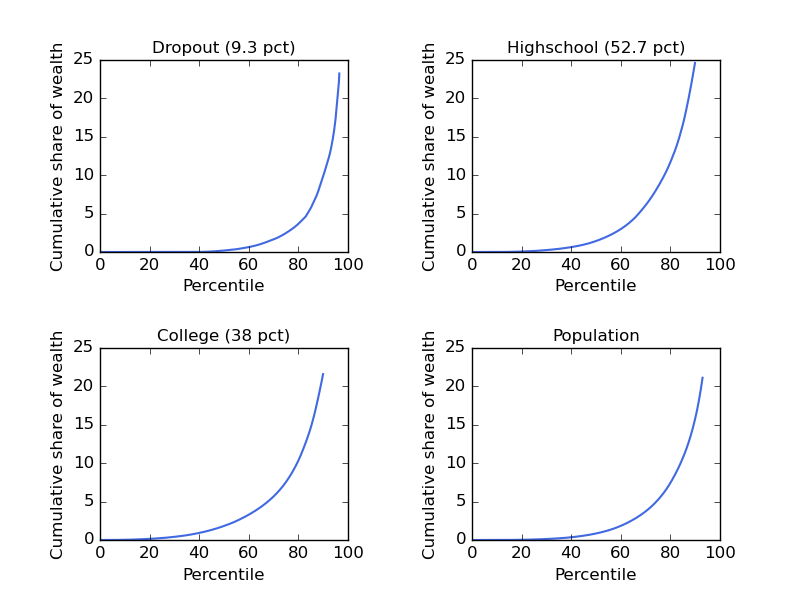
\includegraphics[width=3.5in]{\FigDir/LorenzPoints_dataOnly}
\end{frame}

\begin{frame}
	\frametitle{Consistent with data 2: iMPC from FHN (2021) \\ 
	\small Modelling device: `Splurge' in consumption \normalsize}
	\centering
	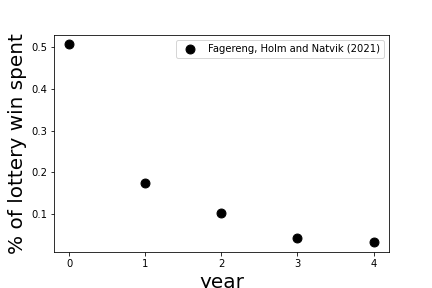
\includegraphics[width=3in]{\econtexRoot/Code/HA-Models/Target_AggMPCX_LiquWealth/Figures/AggMPC_LotteryWin_DataOnly}
	\begin{itemize}
	\itemsep = 0.5\bigskipamount
	\item Auclert, Rognlie and Straub (2018): Also cite FHN for evidence on iMPCs
	\end{itemize}
\end{frame}

%\begin{frame}
%	\frametitle{Approach: Splurge, IMPC, Model and Simulations}
%	\begin{itemize}
%	\itemsep = .5\bigskipamount 
%	\item 
%	\end{itemize}
%\end{frame}

\begin{frame}
\frametitle{Preview of results}
\begin{itemize}
\itemsep = \bigskipamount 
\item Welfare measure: Extension of UI benefits is the clear winner 
	\begin{itemize}
	\itemsep = .25\bigskipamount 
	\item Targeted at individuals with high MPCs 
	\item They also tend to have high MU of consumption 
	\item But: higher spending may continue after recession is over 
	\end{itemize}
\item Spending multiplier: Stimulus check has the highest multiplier 
	\begin{itemize}
	\itemsep = .25\bigskipamount 
	\item Not well targeted, but increases income immediately 
	\item Spending happens during recession 
	\item Also: more easily scaled up 
	\end{itemize}
\item Tax cut: both poorly targeted and substantial amount of income boost may occur after the recession is over
\end{itemize}
\end{frame}

\begin{frame}
\frametitle{Related literature}
\small
\begin{itemize}
	\item \textbf{Effects of transitory income shocks}: 
	Parker, Souleles, Johnson and McClelland (2013); Broda and Parker (2014); Fagereng, Holm and Natvik (2021); Ganong, Greig, Noel, Sullivan and Vavra (2022)
	\item \textbf{HA models consistent with high MPCs}: 
	Kaplan and Violante (2014); Auclert, Rognlie and Straub (2018); Carroll, Crawley, Slacalek and White (2020); Kaplan and Violante (2022) 
	\item \textbf{State dependent multipliers (ZLB)}: 
	Christiano, Eichenbaum and Rebelo (2011); Eggertson (2011); Ramey and Zubairy (2018); Hagedorn, Manovskii and Mitman (2019) 
	\item \textbf{Welfare measures in HA models}:
	Bhandari, Evans, Golosov and Sargent (2021); D{\'a}vila and Schaab (2022)
	\item \textbf{Extended unemployment insurance}:
	Ganong, Greig, Noel, Sullivan and Vavra (2022); Kekre (2022) 
	\item \textbf{High MPCs and impatience}: Parker (2017)
\end{itemize}
\normalsize
\end{frame}

\section{Model}

\begin{frame}
\frametitle{Consumer problem}
\begin{itemize}
	\itemsep = .5\bigskipamount 
	\item Education groups $e(i)$: "Dropout", "Highschool", "College" \\[1ex] 
	\ra\ different distributions of subjective discount factors $\beta_i$
	\item Stochastic income process $\mathbf{y}_{i,t}$
	\item An exogenously given fraction of income is consumed directly (the `splurge')
		\begin{align}
		\mathbf{c}_{sp,i,t} = \varsigma \mathbf{y}_{i,t}
		\end{align}
	\item Given the splurge, remaining consumption $c_{opt,i,t}$ is chosen to to maximize the perpetual-youth lifetime expected-utility
		\begin{align}
		\sum_{t=0}^{\infty}\beta_i^t (1-D)^t \mathbb{E}_0 u(\mathbf{c}_{opt,i,t}).
		\end{align}
		where $D$ is the end-of-life probability and $u(\cdot)$ is a standard CRRA utility function	
\end{itemize}
\end{frame}

\begin{frame}
\frametitle{Consumer problem - Part II}

	\begin{itemize}
		\item The optimization is subject to the budget constraint, given existing market resources $\mathbf{m}_{i,t}$ and income state, and a no-borrowing constraint: 
		\begin{align}
		\mathbf{a}_{i,t} &= \mathbf{m}_{i,t} - \mathbf{c}_{sp,i,t} - \mathbf{c}_{opt,i,t} \\
		\mathbf{m}_{i,t+1} &= R \mathbf{a}_{i,t} + \mathbf{y}_{i,t+1}, \\
		\mathbf{a}_{i,t} &\geq 0,   \notag
		\end{align}
		where $R$ is the gross interest factor.
	\end{itemize}



\end{frame}


\begin{frame}
\frametitle{ Income process}

	\begin{itemize}
		\itemsep = .5\bigskipamount 
		\item Income subject to permanent, transitory, and unempl. shocks
		\item "Permanent income" $p$ evolves according to
		\begin{align}
		\mathbf{p}_{i,t+1} = \psi_{i,t+1}\Gamma_{e(i)}\mathbf{p}_{i,t},
		\end{align}
	 	$\psi_{i,t+1}$: shock to permanent income \\[.7ex]
	 	$\Gamma_{e(i)}$: educaton-specific average growth rate of income 
		\item Total income s.t. transitory shock $\xi_{i,t}$ and  employment status
		\begin{align}
		\mathbf{y}_{i,t} =   \begin{cases}
		\xi_{i,t}\mathbf{p}_{i,t}, & \text{if employed} \\
		\rho_b \mathbf{p}_{i,t}, & \text{if unemployed with benefits} \\
		\rho_{nb} \mathbf{p}_{i,t}, & \text{if unemployed without benefits} 
		\end{cases}
		\end{align}
		where $\rho_x$ are the status-specific replacement rates.
	\end{itemize}

\end{frame}


\begin{frame}
\frametitle{ Employment status and recessions}
\begin{itemize}
	\itemsep = \bigskipamount 
	\item Emplyoment status is subject to a Markov process
	\begin{itemize}
		\itemsep = .5\bigskipamount
		\item Employed consumer: continue being employed or become unemployed 
		\item Unemployed consumers: receives benefits for two quarters
	\end{itemize}

	\item Recession is given by an MIT shock
	\begin{itemize}
		\itemsep = .5\bigskipamount
		\item Unemployment rate doubles in each education group
		\item Expected length of unemployment increases from 2 to 4q
		\item End of recession occurs as a Bernoulli process calibrated for an avg. rec. length of 6q
	\end{itemize}
\end{itemize}
\end{frame}

\begin{frame}
	\frametitle{Aggregate demand effects \\ 
	\small (as in Krueger, Mitman and Perri, 2016) \normalsize}
	\begin{itemize}
		\itemsep = .5\bigskipamount 
		\item Baseline: No feedback from aggregate consumption to income
		\item Extension: We allow for aggregate demand effects from consumption on income during the recession
		
		\item The AD effect is given by
		\begin{align}
			AD(C_t) =   \begin{cases}
				\Big(\frac{C_t}{\tilde{C}}\Big)^\kappa, & \text{if in a recession} \\
				1, & \text{otherwise} ,
			\end{cases}
		\end{align}
		where $\tilde{C}$ is the level of consumption in the steady state. 
		
		\item Idiosyncratic income in the extension model is then given by
		\begin{align}
			\mathbf{y}_{AD,i,t} = AD(C_t)\mathbf{y}_{i,t}.
		\end{align}
	\end{itemize}
\end{frame}

\begin{frame}
\frametitle{Three policies to fight the recession}

	\begin{itemize}
	\itemsep =.5\bigskipamount
	\item Stimulus check
	\begin{itemize}
		\itemsep = .25\bigskipamount 
		\item Everyone receives a check for \$1,200 in q1 of the recession
		\item Check is means-tested: Full check if perm. income $\leq$ \$100k; Falls linearly for higher incomes and zero for those $\geq$ \$150k
	\end{itemize}

	\item Extended unemployment benefits
	\begin{itemize}
		\itemsep = .25\bigskipamount 
		\item Unemployment benefits are extended from 2 to 4 q
		\item Extension occurs regardless of whether recession ends
	\end{itemize}

	\item Payroll tax cut
	\begin{itemize}
		\item Employees payroll tax rate is reduced such that income rises by 2\% for 8q	
	\end{itemize}
\end{itemize}
\medskip
\hrule \medskip
\begin{itemize}
	\itemsep = .5\bigskipamount
	\item For welfare measure: Compare policies of equal cost
	\item Policies are debt-financed and repayed after the short recessions we focus on
\end{itemize}
\end{frame}

\section{Parametrization}

\begin{frame}
\frametitle{Parametrization --- Strategy}
\begin{itemize} 
\itemsep = \bigskipamount 
\item First: Estimate the splurge factor in a Norwegian version of the economy --- match iMPCs from FHN (2021)
\item Calibrate a set of parameters that affect all education groups equally 
\item Calibrate a set of parameters that match features of the different education groups 
\item Estimate a discount factor distribution for each education group to match within-group distribution of liquid wealth
	\begin{itemize}
	\itemsep = .25\bigskipamount 
	\item $\beta_e$: center of discount factor distribution
	\item $\nabla_e$: spread of discount factor distribution 
	\item Uniform distribution, approximated with 7 different types
	\end{itemize}
\end{itemize} 
\end{frame}

\begin{frame}
	\frametitle{iMPC from FHN (2021)}
	\centering 
%	\includegraphics[width=3in]{\FigDir/AggMPC_LotteryWin}
	\includegraphics[width=3in]{\econtexRoot/Code/HA-Models/Target_AggMPCX_LiquWealth/Figures/AggMPC_LotteryWin}
	\begin{itemize}
		\itemsep = .5\bigskipamount 
		\item Estimated splurge factor: $\varsigma = 0.31$
		\item Robustness exercise: How close do we get and what are our results if we set $\varsigma = 0$? To be computed\ldots 
	\end{itemize}
\end{frame}

\begin{frame}
\frametitle{Parameters --- same for all types}
   \begin{tabular}{lcd{3}} 
	\toprule
	\multicolumn{3}{l}{Parameters that apply to all types} \\ \midrule
	Parameter & Notation & \text{Value} \\ \midrule 
	Risk aversion & $\gamma$ & 2.0 \\ 
	Splurge & $\varsigma$ & 0.307 \\ 
	Survival probability, quarterly & $1-D$ & 0.994 \\
	Risk free interest rate, quarterly (gross) & $R$ & 1.01 \\ 
	Standard deviation of transitory shock & $\sigma_\xi$ & 0.346 \\
	Standard deviation of permanent shock & $\sigma_\psi$ & 0.0548 \\ 
	Unemployment benefits replacement rate (share of PI) & \only<1>{$\rho_b$}\only<2>{\textcolor{red}{$\rho_b$}} &
	\only<1>{0.7}\only<2>{\textcolor{red}{0}.\textcolor{red}{7}} \\ 
	Unemployment income w/o benefits (share of PI) & \only<1>{$\rho_{nb}$}\only<2>{\textcolor{red}{$\rho_{nb}$}} & \only<1>{0.5}\only<2>{\textcolor{red}{0}.\textcolor{red}{5}} \\ 
	Avg. duration of unemp. benefits in normal times (quarters) & & 2 \\
	Avg. duration of unemp. spell in normal times (quarters) & & 1.5 \\
	Probability of leaving unemployment & $\pi_{ue}$ & 0.667 \\ 
	Consumption elasticity of aggregate demand effect & $\kappa$ & 0.3 
	\\ \bottomrule 
\end{tabular}
\end{frame}

\begin{frame}
\frametitle{Parameters --- by education group \hyperlink{sli:policies}{\beamerbutton{Policy parameters}}}
\label{sli:paramsByEd}
\begin{tabular}{lccc}
	\toprule 
	\multicolumn{4}{l}{Parameters calibrated for each education group} \\ \midrule
	& Dropout & Highschool & College \\ \midrule
	Percent of population & \phantom{0}9.3 & 52.7 & 38.0 \\ 
	Avg. quarterly PI of ``newborn'' agent (\$1000) & \phantom{0}6.2 & 11.1 & 14.5 \\
	Std. dev. of $\log($PI$)$ of ``newborn'' agent & 0.32 & 0.42 & 0.53 \\
	Avg. quarterly gross growth rate of PI ($\Gamma_e$) & 1.0036 & 1.0045 & 1.0049 \\
	Unemployment rate in normal times (percent) & \phantom{0}8.5 & \phantom{0}4.4 & \phantom{0}2.7 \\ 
	Probability of entering unemployment ($\pi_{eu}^{e}$, percent) & \phantom{0}6.2 & \phantom{0}3.1 & \phantom{0}1.8 
	\\ \bottomrule 
\end{tabular}
\end{frame}

\begin{frame}
\begin{tabular}{lccc}
	\multicolumn{4}{l}{Estimated discount factor distributions} \\ 
	& Dropout & Highschool & College \\ \midrule
	$(\beta_e, \nabla_e)$ & (0.694, 0.542) & (0.904, 0.099) & (0.978,0.015) \\
	(Min, max) in approximation & (0.230, 0.995) & (0.819, 0.989) & (0.965, 0.991) \\
	\midrule 
\end{tabular} 
\begin{tabular}{lccc}
	\multicolumn{4}{l}{ } \\ \midrule
	\textbf{Estimation targets} & Dropout & Highschool & College \\ \midrule
	Median LW/ quarterly PI (data, percent) & 4.64 & 30.2 & 112.8 \\ 
	Median LW/ quarterly PI (model, percent) & 4.64 & 30.2 & 112.8 %\\
	%         $[20,40,60,80]$ pctiles of Lorenz curve (data) & $[0, 0.01, 0.6, 3.6]$ & $[0.06, 0.6, 3.0, 11.6]$ & $[0.2, 0.9, 3.3, 10.3]$ \\
	%         $[20,40,60,80]$ pctiles of Lorenz curve (model) & $[0.0, 0.0, 0.5, 3.6]$ & $[0.04, 0.9, 3.7, 11.3]$ & $[0.3, 1.5, 4.0, \phantom{0}9.9]$
	\\ \midrule 
\end{tabular} 
\begin{tabular}{lcccc}
	\multicolumn{5}{l}{ } \\ \midrule
	\textbf{Non-targeted moments} & Dropout & Highschool & College & Population \\ \midrule
	Percent of total wealth (data) & 0.8 & 17.9 & 81.2 & 100 \\
	Percent of total wealth (model) & 12.4 & 18.6 & 69.0 & 100 \\
	Avg. annual MPC (model, incl. splurge) & 0.79 & 0.78 & 0.54 & 0.69
	\\ \bottomrule 
\end{tabular}
\end{frame}




\begin{frame}
\frametitle{SCF liquid wealth}
\centering
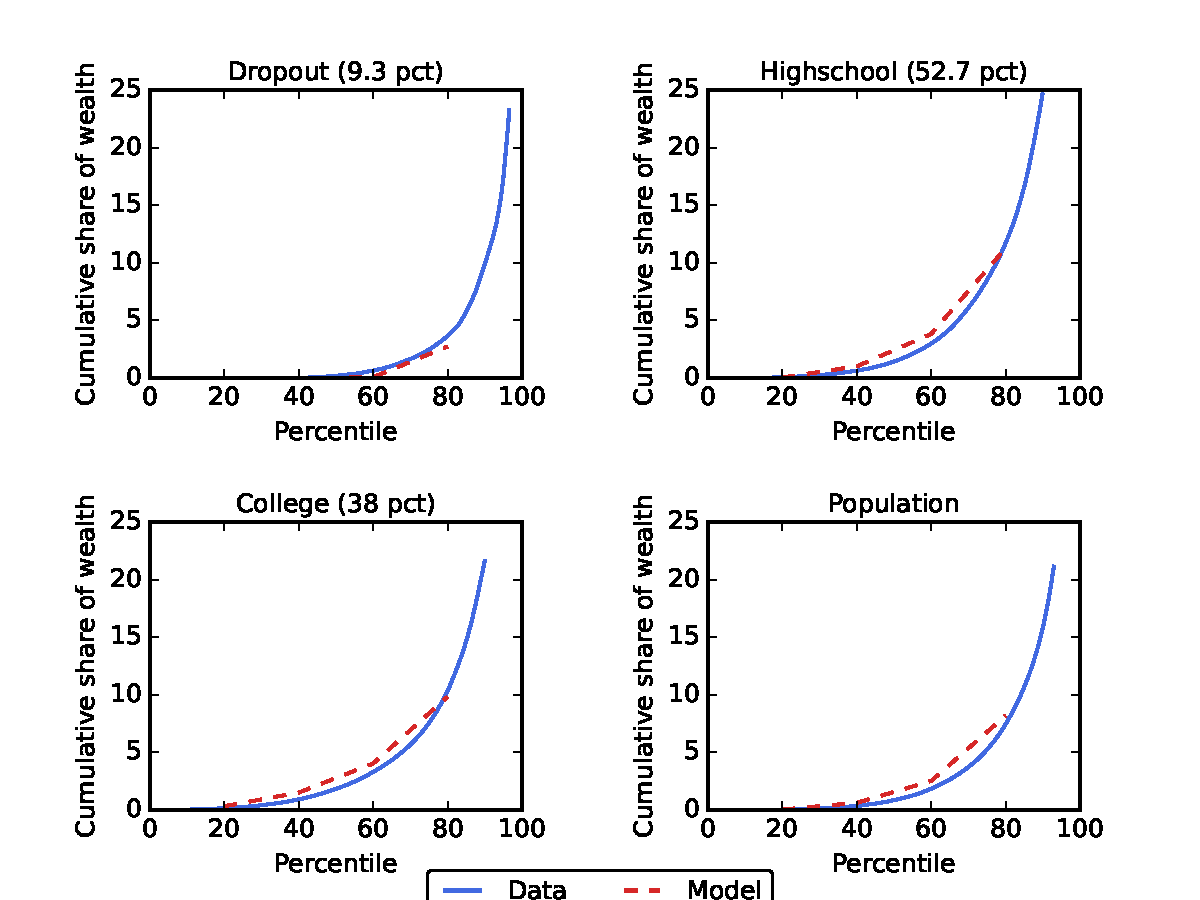
\includegraphics[width=4in]{\FigDir/LorenzPoints}
\end{frame}



\section{Results}


\begin{frame}
\frametitle{IRFs for stimulus check}
\centering
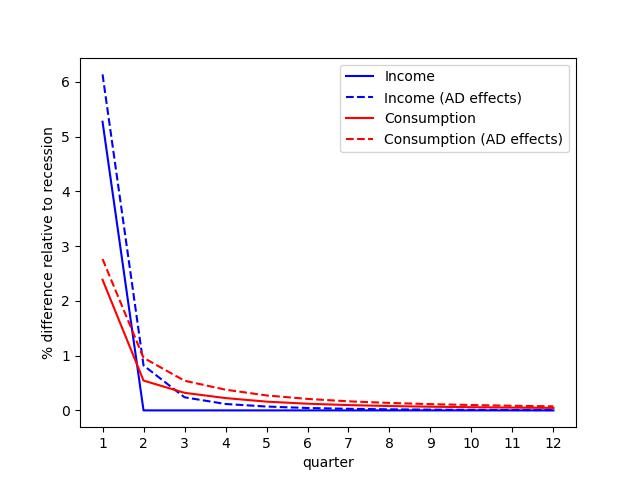
\includegraphics[width=0.6\linewidth]{\econtexRoot/Code/HA-Models/FromPandemicCode/Figures/recession_Check_relrecession}
\begin{itemize}
	\itemsep = .5\bigskipamount 
	\item W/o AD effects: Q1 income is 5.5\% higher; consumption jumps by 3\% 
	\item With AD effects: Q1 income is 6.5\% higher; consumption elevated for longer time
\end{itemize}
\end{frame}


\begin{frame}
\frametitle{IRfs for extension of unemployment benefits}
	\centering
	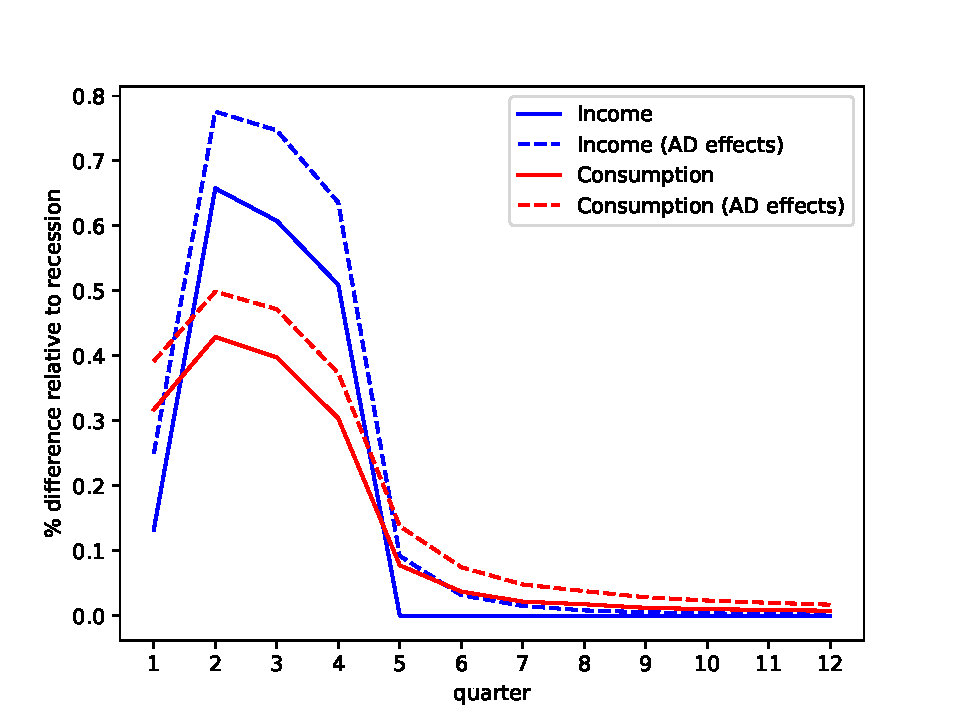
\includegraphics[width=0.6\linewidth]{Code/HA-Models/FromPandemicCode/Figures/recession_UI_relrecession}
\begin{itemize}
	\itemsep = .5\bigskipamount 
	\item W/o AD effects: quarterly income increases by max 0.7 percent, consumption response shows anticipation of longer duration
	\item With AD effects: extra boost to income by 0.2 percent, consumption stays elevated for longer time
\end{itemize}

\end{frame}

\begin{frame}
\frametitle{IRFs for payroll tax cut}
	\centering
	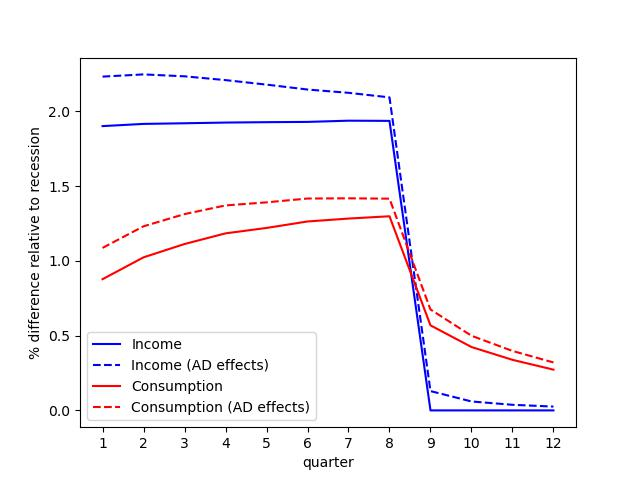
\includegraphics[width=0.6\linewidth]{Code/HA-Models/FromPandemicCode/Figures/recession_taxcut_relrecession}

\begin{itemize}
	\itemsep = .5\bigskipamount 
	\item W/o AD effects: income rises by close to 2 percent; Consumption jumps by 1.5 percent and drops sharply after the income decline.
	\item With AD effects, income rises by 2.5 percent, declines steadily as the recession's likelihood decreases
\end{itemize}
\end{frame}


\begin{frame}
\frametitle{Multipliers when aggregate demand effects are present}
\begin{equation*}
M^P_t = \frac{\text{Net present value of policy-induced consumption up to $t$}}{\text{Net present value of the cost of the policy}}
\end{equation*}
\centering
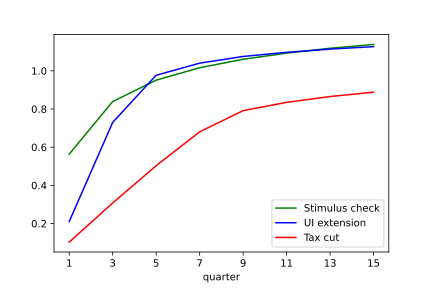
\includegraphics[width=0.5\linewidth]{Code/HA-Models/FromPandemicCode/Figures/Cummulative_multipliers}
\footnotesize
\begin{tabular}{@{}lccc@{}} 
	& Tax Cut    & UI extension    & Stimulus check    \\ 
	Long-run Multiplier  &1.079  & 1.275  & 1.339     \\ 
	Policy expenditure during recession  &57.6\%  & 80.6\%  & 100.0 \%    \\ 
\end{tabular}  
\normalsize 
\end{frame}

\begin{frame}
\frametitle{Welfare measure construction}

	Guiding principles
	
	\begin{enumerate}
		\item Each consumer is valued equally by the social planner 
		\item Utility from splurge in the same way as other spending
		\item No social benefit to the policies outside of a recession
	\end{enumerate} 
	
	\vspace{0.6cm}
	
	Simple aggregation of consumer util. only satisfies principle 1 \& 2:
	\begin{align*}
	\mathcal{W}(\text{policy},Rec,AD) =\frac{1}{N}\sum_{i=1}^{N} \sum_{t=0}^{\infty} \beta_S^t u(\mathbf{c}_{it,\text{policy},Rec,AD}) 
	\end{align*}
	
	\begin{itemize}
		\item $\mathbf{c}_{it,\text{policy},Rec,AD}$: consumption paths (including splurge) for each consumer / policy
		\item $Rec\in\{1,0\}$: recession indicator, $AD\in\{1,0\}$: AD ind.
		\item $\beta_S = 1/R$: social planner's discount factor 
	\end{itemize}	

\end{frame}


\begin{frame}
\frametitle{Welfare measure construction II}

	To satisfy principle 3 we define $\mathcal{C}(\text{policy},Rec,AD) =$
	\begin{align*}
	& \bigg( \underbrace{\frac{\mathcal{W}(\text{policy},Rec,AD)-\mathcal{W}(\text{None},Rec,AD)}{\mathcal{W}^c}}_\text{\RNum{1}}  - \underbrace{\frac{PV(\text{policy},Rec)}{\mathcal{P}^c} }_\text{\RNum{2}} \bigg) \nonumber \\  
	& -
	\bigg( \underbrace{\frac{\mathcal{W}(\text{policy},0,0) - \mathcal{W}(\text{None},0,0)}{\mathcal{W}^c}}_\text{\RNum{3}}  - \underbrace{\frac{PV(\text{policy},0)}{\mathcal{P}^c}}_\text{\RNum{4}}  \bigg) 
	\end{align*}
	
	\begin{itemize}
		\item \RNum{1}: Policy-induced increase in agg. welfare (in bp of SS-cons.)
		\item \RNum{2}: Cost of policy $\Leftrightarrow$ \RNum{1} - \RNum{2}: Net agg. welfare increase
		\item \RNum{3} - \RNum{4}: Net welfare impact of policy outside of recession
		\item $\mathcal{C}$ measures only welfare effects beyond pure redistribution
	\end{itemize}

\end{frame}


\begin{frame}
\frametitle{Welfare results}
\centering 
\begin{tabular}{@{}lccc@{}} 
	\toprule 
	& Check      & UI    & Tax Cut    \\  \midrule 
	$\mathcal{C}(\text{policy},Rec,0)$ & 0.011  & 0.580  & 0.002     \\ 
	$\mathcal{C}(\text{policy},Rec,AD)$ & 0.171  & 1.266  & 0.065     \\ 
\end{tabular}  
\medskip
\begin{itemize}
	\itemsep = .75\bigskipamount 
	\item All policies adjusted to the fiscal size of the UI extension
	\item Interpretation: A welfare gain of x $\Leftrightarrow$ social planner is indifferent between 
	\begin{itemize}
		\itemsep = .25\bigskipamount 
		\item the stimulus policy being implemented in response to a recession and 
		\item a permanent increase in the baseline consumption of the total population by x basis points (0.01\% of baseline cons.)
	\end{itemize}
		\item All policies much more effective when mulitplier present
\end{itemize}
\end{frame}


%\begin{frame}
%\frametitle{Robustness}
%List here all robustness checks performed
%\end{frame}


\begin{frame}
\frametitle{Conclusion: Comparing the policies}
\begin{itemize}
\itemsep = .5\bigskipamount 
\item We have compared three consumption stimulus policies in a HA model consistent with data on the distribution of liquid wealth and intertemporal MPCs 
\item Welfare measure: UI extension is the clear bang-for-the-buck winner 
\item The stiumulus check is less well targeted, but\ldots 
	\begin{itemize}
		\itemsep = .25\bigskipamount 
		\item is transferred immediately ensuring that money arrives when it is most valuable 
		\item is more easily scaled up to provide more stimulus 
	\end{itemize}
\item The tax cut is both poorly targeted and may yield substantial spending after the recession is over 
\item Framework can be used to evaluate other candidate policies 
\item Other (competing?) models to evaluate these policies should match similar features of the data at the micro level 

\end{itemize}

\end{frame}


\section{Appendix}

\begin{frame}
\frametitle{Parameters describing the policies \hyperlink{sli:paramsByEd} {\beamerbutton{Back}}}
\label{sli:policies}
\centering 
\begin{tabular}{lc}
	\toprule 
	\multicolumn{2}{l}{Parameters describing policy experiments} \\ \midrule 
	Parameter & Value \\ \midrule 
	Change in unemployment rates in a recession & $\times 2$ \\ 
	Expected unemployment spell in a recession & 4 quarters \\ 
	Average length of recession & 6 quarters \\ 
	Size of stimulus check & \$1,200 \\ 
	PI threshold for reducing check size & \$100,000 \\ 
	PI threshold for not receiving check & \$150,000 \\ 
	Extended unemployment benefits & 4 quarters \\
	Length of payroll tax cut & 8 quarters \\ 
	Income increase from payroll tax cut & 2 percent \\ 
	Belief (probability) that tax cut is extended & 50 percent 		
	\\ \bottomrule
\end{tabular} 
\end{frame}

\begin{frame}
\frametitle{Robustness: Different replacement rates}
\centering    
\begin{itemize}
	\item Discount factor distributions: 
\end{itemize}
\small
\begin{tabular}{llc|cccccc} 
	\toprule
	& & & \multicolumn{2}{c}{Dropout} & \multicolumn{2}{c}{Highschool} & \multicolumn{2}{c}{College} \\ \midrule 
	& & Splurge & $\beta$ & $\nabla$ & $\beta$ & $\nabla$ & $\beta$ & $\nabla$ \\ \midrule 
	Basel. & ($\rho_{b}=0.7$, $\rho_{nb}=0.5$) & 0.307 & 0.694 & 0.542 & 0.904 & 0.099 & 0.978 & 0.015 \\ 
	Alt. & ($\rho_{b}=0.3$,  $\rho_{nb}=0.15$) & 0.307 & 0.599 & 0.687 & 0.852 & 0.159 & 0.968 & 0.028
	\\ \bottomrule 
\end{tabular}
\normalsize
\begin{itemize}
\item Welfare results: 
\end{itemize}
\small
\begin{tabular}{@{}lllll@{}}
	\toprule
	&                    & Stimulus check & UI extension & Tax cut \\ \cmidrule(l){1-5} 
	\multirow{2}{*}{no AD effects} 	& Baseline  ($\rho_{b}=0.7$, $\rho_{nb}=0.5$) 		& 0.011          & 0.580        & 0.002   \\
	& Altern.  ($\rho_{b}=0.3$, $\rho_{nb}=0.15$) 	& 0.043          & 1.913        & 0.003   \\ \cmidrule(l){1-5} 
	\multirow{2}{*}{AD effects}		& Baseline  ($\rho_{b}=0.7$, $\rho_{nb}=0.5$)    	& 0.171          & 1.266        & 0.065   \\
	& Altern.  ($\rho_{b}=0.3$, $\rho_{nb}=0.15$)    & 0.169          & 2.620        & 0.052   \\ \cmidrule(l){1-5} 
\end{tabular}
\normalsize
\end{frame}

\begin{frame}
\frametitle{Robustness: Different interest rates}
    \begin{tabular}{lc|cccccc} 
	\toprule
	& & \multicolumn{2}{c}{Dropout} & \multicolumn{2}{c}{Highschool} & \multicolumn{2}{c}{College} \\ \midrule 
	& Splurge & $\beta$ & $\nabla$ & $\beta$ & $\nabla$ & $\beta$ & $\nabla$ \\ \midrule 
	$R = 1.005$ & 0.307 & 0.701 & 0.520 & 0.909 & 0.099 & 0.983 & 0.014 \\
	$R = 1.01$ (baseline) & 0.307 & 0.694 & 0.542 & 0.904 & 0.099 & 0.978 & 0.015 \\ 
	$R = 1.015$ & 0.307 & 0.691 & 0.542 & 0.899 & 0.099 & 0.973 & 0.016 
	\\ \bottomrule 
\end{tabular}
\end{frame}


\end{document}

